Experiments for the segmentation procedure were carried out for the two proposed methods: a) FFT and b) STFT. The proposed image sets were built in order to perform tests with real multifocus microscopy images with their own point spread function and defocus blur feature. The coin images were acquired with 300x magnification,  5 $\mu m$ Depth of Field and 10 $\mu m$ step between each image on the $z$ axis. Two different slopes between the coin letters were considered: the slope between the background of the coin and the "o" letter and the same approach for the 90 degrees rotated "v" letter in the Portuguese word \emph{centavos} of the coin, shown in figure \ref{fig:original_coin}. The slope on the images was made on purpose for creating a very pronounced blur effect with the differences in the microscope objective's height. Ten images were taken from the "o" and "v" slopes. The blurred parts are known to be either \emph{left} or \emph{right}, as summarized by table \ref{tab:coin_card_set_description} and shown in figure \ref{fig:card_coin_images}:

\begin{figure}[H]
	\centering
	\caption{\label{fig:original_coin}10-\emph{cent} Brazilian Real coin.}
	\begin{center}
	    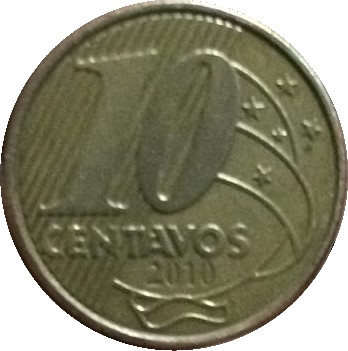
\includegraphics[scale=0.5, trim = {0 0 0 1cm}]{images/fig16.png}
	\end{center}
	\centering
    \fautor
\end{figure}

\begin{table}[H]
    \centering
    \caption{Description of the sharp parts of the image sets (a) coin "o" letter and (b) coin "v" letter.}\label{tab:coin_card_set_description}
    \begin{subtable}{.35\linewidth}
    
    %Center the table
		\begin{center}
		% Title of the table
		\caption{}
        \begin{tabular}
        {|c|c|c|}
        \hline
        
            % header
            Image & Sharp Part
            \\ \hline
            % data
            coin "o" 1 & None
            \\ \hline
            
            coin "o" 2 & None
            \\ \hline
            
            coin "o" 3 & Left
            \\ \hline
            
            coin "o" 4& Left
            \\ \hline
            
            coin "o" 5 & Left
            \\ \hline
            
            coin "o" 6 & Right
            \\ \hline
            
            coin "o" 7 & Right
            \\ \hline
            
            coin "o" 8 & None
            \\ \hline
            
            coin "o" 9 & None
            \\ \hline
            
            coin "o" 10 & None
            \\ \hline
            
        \end{tabular}
    \end{center}
    \end{subtable}%
    \begin{subtable}{.35\linewidth}

        %Center the table
		\begin{center}
		% Title of the table
		\caption{}
        \begin{tabular}
        {|c|c|c|}
        \hline
        
            % header
            Image & Sharp Part
            \\ \hline
            % data
            coin "v" 1 & None
            \\ \hline
            
            coin "v" 2 & None
            \\ \hline
            
            coin "v" 3 & Right
            \\ \hline
            
            coin "v" 4& Right
            \\ \hline
            
            coin "v" 5 & Right
            \\ \hline
            
            coin "v" 6 & Right
            \\ \hline
            
            coin "v" 7 & Left
            \\ \hline
            
            coin "v" 8 & Left
            \\ \hline
            
            coin "v" 9 & Left
            \\ \hline
            
            coin "v" 10 & Left
            \\ \hline
            
        \end{tabular}
    \end{center}
    \end{subtable} 
    \hspace{0.8cm}
    \fautor
\end{table}

\begin{figure}[H]
	\centering
	\caption{\label{fig:card_coin_images}Samples from the coin and card image sets: (a) and (b) left and right sharp sides of coin "o" letter, respectively, (c) and (d) left and right sharp sides of coin "v" letter, respectively.}
	\begin{center}
	    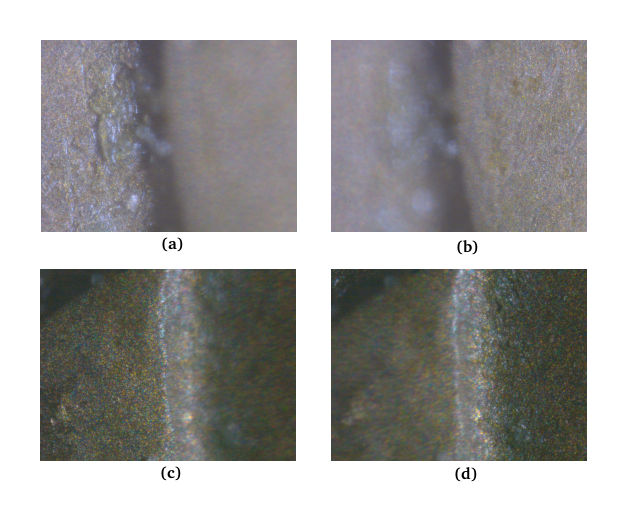
\includegraphics[scale=0.6, trim = {0 1cm 0 1cm}]{images/fig17.png}
	\end{center}
	\centering
    \fautor
\end{figure}

\noindent An analogous image set for testing purposes was created, i.e. the card. It consists of images of a contact pad for the electrical interface of a bank card. It was chosen because of a coarser slope when compared to the coin images. The images were acquired also with 300x magnification, a 5 $\mu m$ Depth of Field and a 10 $\mu m$ step between each image on the $z$ axis. Some samples of the card image set are denote by figure \ref{fig:card_set_images} and the description of the card set can be seen in table \ref{tab:card_set_description}.

\begin{figure}[H]
	\centering
	\caption{\label{fig:card_set_images}Card contact pad images: contact pad (a), left and right sharp sides (b) .}
	\begin{subfigure}{.5\textwidth}
        \centering
        \frame{
\includegraphics[scale=1]{images/fig18a.png}}
        \caption{}
    \end{subfigure}\\
    \begin{subfigure}{\textwidth}
         \centering
         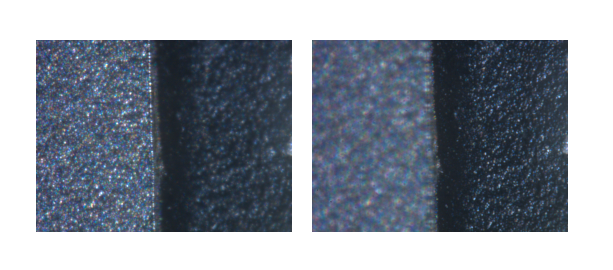
\includegraphics[scale=0.5, trim = {0 0cm 0 0cm}]{images/fig18b.png}
         \caption{}
    \end{subfigure}
	    \fautor
\end{figure}


\begin{table}[htb]
    \centering
    \caption{Description of the sharp parts of the card image set.}\label{tab:card_set_description}
    %Center the table
		\begin{center}
		% Title of the table
        \begin{tabular}
        {|c|c|c|}
        \hline
            % header
            Image & Sharp Part
            \\ \hline
            % data
            card 1 & None
            \\ \hline
            
            card 2 & None
            \\ \hline
            
            card 3 & Left
            \\ \hline
            
            card 4& Left
            \\ \hline
            
            card 5 & Left
            \\ \hline
            
            card 6 & Left
            \\ \hline
            
            card 7 & Right
            \\ \hline
            
            card 8 & Right
            \\ \hline
            
            card 9 & Right
            \\ \hline
            
            card" 10 & Right
            \\ \hline
            
            card" 11 & None
            \\ \hline

            card" 12 & None
            \\ \hline
            
        \end{tabular}
    \end{center}
    \fautor
\end{table}

An artificially blurred image was also used for the tests. The airplane image consists of an common standard $256$x$512$ test image of an F-16 airplane, obtained from the \sigla{USC-SIPI}{University of Southern California - Signal and Image Processing Institute} image databases \cite{uscsipi1977image}. The blurring process consisted of dividing the image in two halves (left and right) with $256$x$512$ pixels each and blurring the left one with a Gaussian Blur Kernel of radius $30$ with the aid of \sigla{GIMP}{GNU Image Manipulation Program}. This image set is shown in figure \ref{fig:airplane_set_images}:

\begin{figure}[H]
	\centering
	\caption{\label{fig:airplane_set_images}Airplane contact pad images: left (a) and right (b) sharp sides.}
	\begin{center}
	    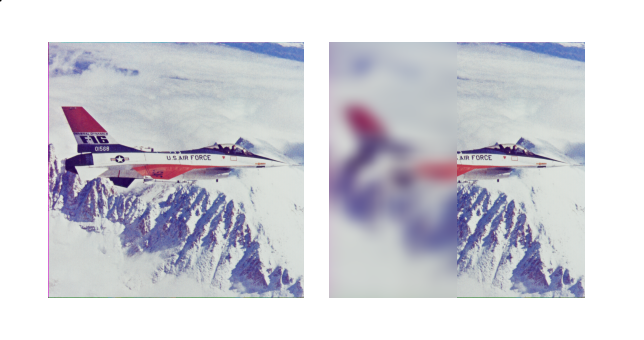
\includegraphics[scale=0.6, trim = {0 1cm 0 1cm}]{images/fig19.png}
	\end{center}
	\centering
    \fautor
\end{figure}

\section{FFT Test}
\label{sec:fft-test}

As expected, the global approach is capable of electing the mostly sharp image within a set of partially blurred images. The magnitude of the spectral energy density values was higher for the sharper images, mostly the ones which have a sharp side, either left or right. Three frequency bands were considered to compute the results: \emph{mid}, \emph{high} and \emph{highest}. The computation of the bands was done in the three proposed colourspaces, and the grayscale one was the most precise. Comprehensive results for grayscale and other colourspaces are shown in appendix \ref{chapter:fft-test-results}. Notice that this approach is not capable of precisely pointing out the location of the blurry parts of the image. Figure \ref{fig:fft_results} presents the frequency band energy values with the grayscale colourspace on each band for the FFT approach. The amount of bar triads is related to the amount of images in the set: for the coin "o" and coin "v" images, 10 bar triads were shown; analogously, 12 for the card set and 2 for the airplane set.

\begin{figure}[H]
    \centering
    \caption{\label{fig:fft_results}Grayscale colourspace FFT approach for coin "o" (upper left), coin "v" (upper right), card (lower left) and airplane (lower right) images.}
    \subfloat{
        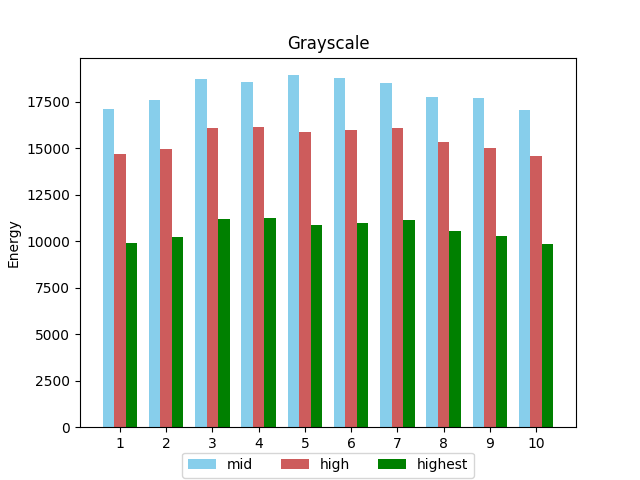
\includegraphics[width=0.45\textwidth]{images/fig20a.png}
        \label{fig:subfig1}
    }
    \qquad
    \subfloat{
        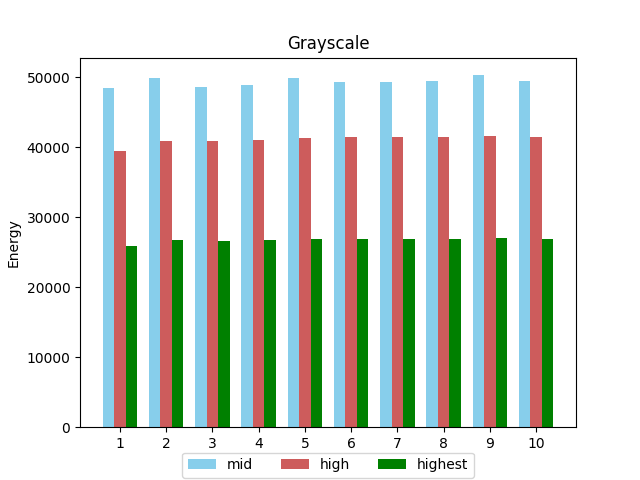
\includegraphics[width=0.45\textwidth]{images/fig20b.png}
        \label{fig:subfig2}
    }
    \subfloat{
        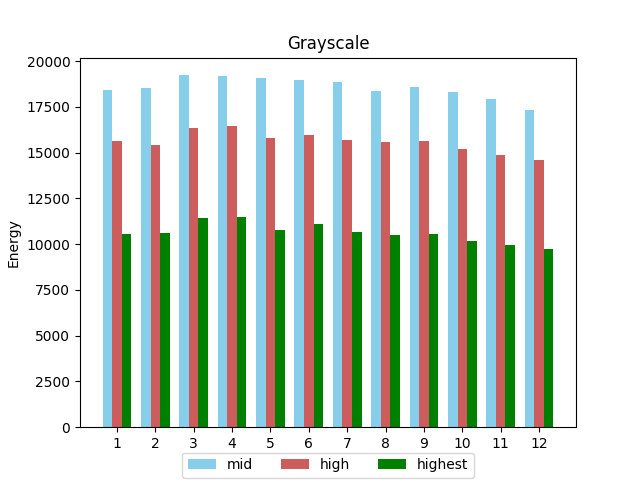
\includegraphics[width=0.45\textwidth]{images/fig20c.png}
        \label{fig:subfig3}
    }
    \qquad
    \subfloat{
        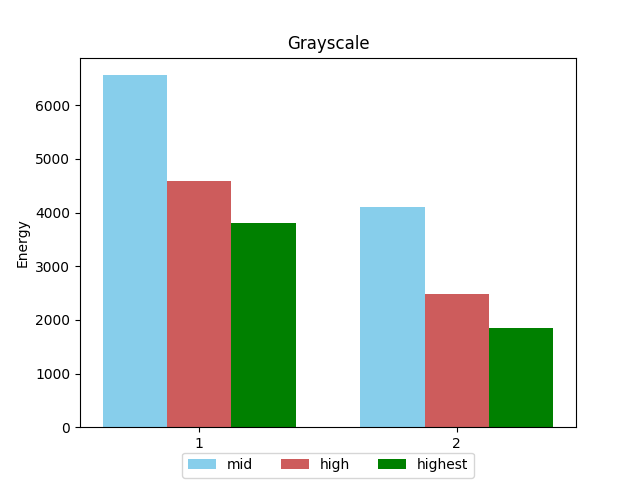
\includegraphics[width=0.45\textwidth]{images/fig20d.png}
        \label{fig:subfig4}
    }
    \hspace{1cm}
    \fautor
\end{figure}

\section{STFT Test}

The Short-time Fourier Transform approach presented relevant results concerning the information about the amount of blur on each region of the images. The test cases were made in such a way that positive results should be expected: the most efficient window size was already set due to the prior knowledge about the blurry and the sharp regions. With the same configuration for colourspaces and frequency bands, the test were done with several different window functions that are printed on the appendix \ref{chapter:stft-test-results}. The figures \ref{fig:stft_card}, \ref{fig:stft_coin_o}, \ref{fig:stft_coin_v} and \ref{fig:stft_airplane} presents the frequency band energy values with the grayscale colourspace on each band for the STFT approach, with the Hann window function, for the left and right sections (left and right in the airplane graph and \emph{L} and \emph{R} for the other graphs). The graphs stand for the card, coin "o", coin "v" and airplane image sets, respectively. The bar triad settings are the same as in section \ref{sec:fft-test}.


\begin{figure}[ht]
	\centering
	\caption{\label{fig:stft_card}Grayscale colourspace STFT approach for card images.}
	\begin{center}
	    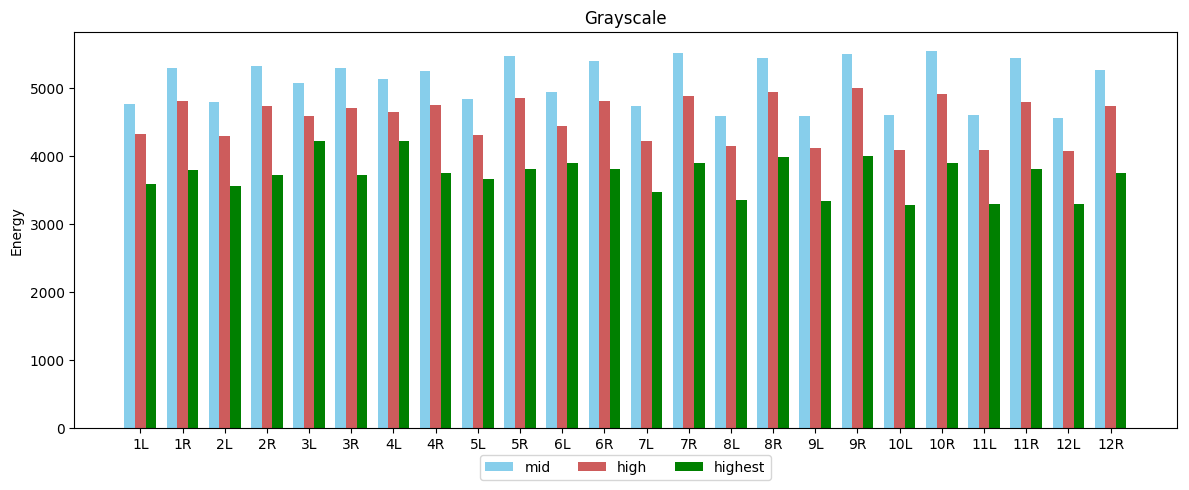
\includegraphics[scale=0.52, trim = {0 1cm 0 1cm}]{images/fig21.png}
	\end{center}
	\centering
    \fautor
\end{figure}

\begin{figure}[ht]
	\centering
	\caption{\label{fig:stft_coin_o}Grayscale colourspace STFT approach for coin "o" images.}
	\begin{center}
	    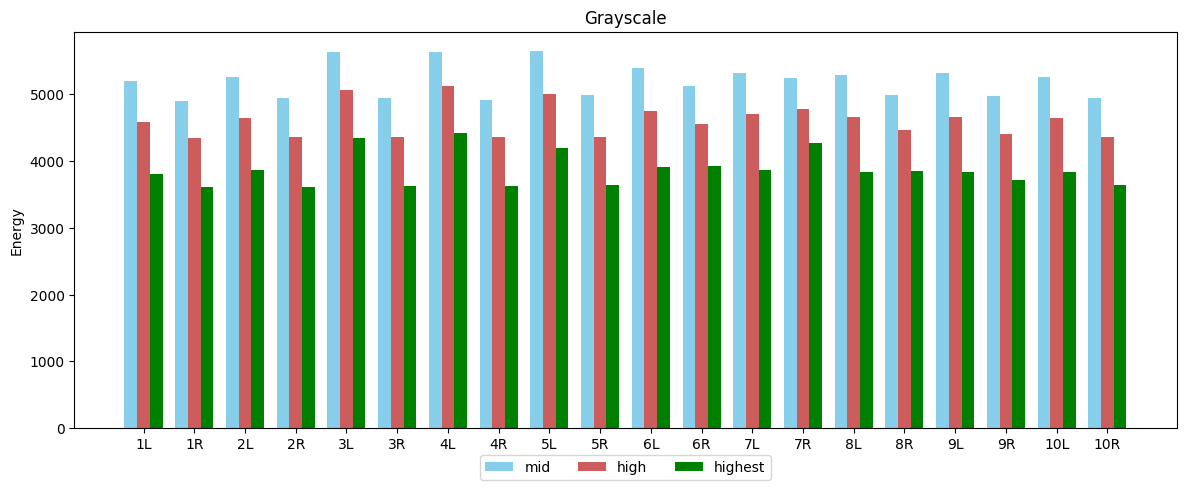
\includegraphics[scale=0.52, trim = {0 1cm 0 1cm}]{images/fig22.png}
	\end{center}
	\centering
    \fautor
\end{figure}

\begin{figure}[ht]
	\centering
	\caption{\label{fig:stft_coin_v}Grayscale colourspace STFT approach for coin "v" images.}
	\begin{center}
	    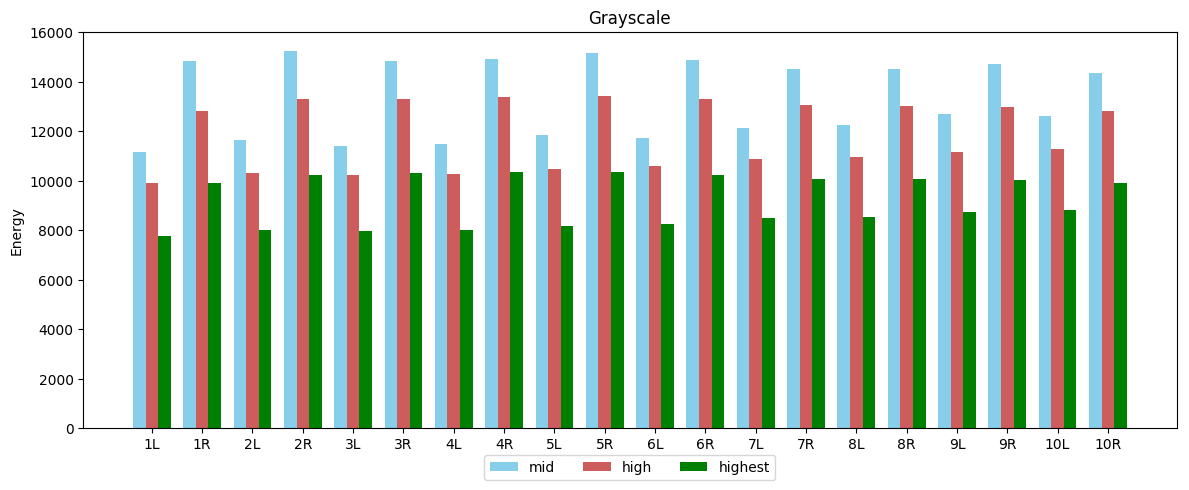
\includegraphics[scale=0.52, trim = {0 1cm 0 1cm}]{images/fig23.png}
	\end{center}
	\centering
    \fautor
\end{figure}

\begin{figure}[ht]
	\centering
	\caption{\label{fig:stft_airplane}Grayscale colourspace STFT approach for airplane images.}
	\begin{center}
	    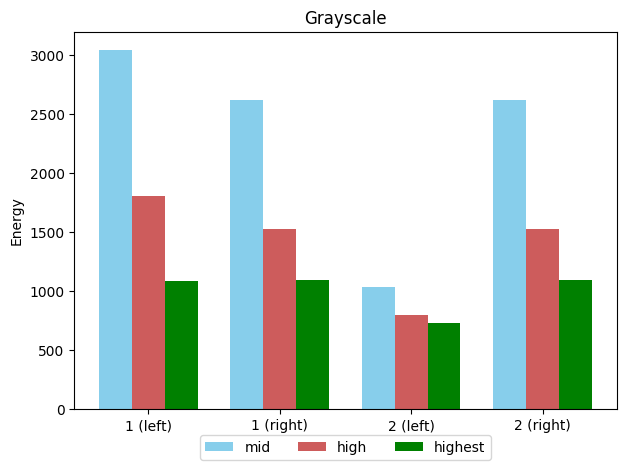
\includegraphics[scale=0.6, trim = {0 1cm 0 1cm}]{images/fig24.png}
	\end{center}
	\centering
    \fautor
\end{figure}

\noindent The above graphs show that the magnitude of the energy levels on blurry sections is lower than the same metric for the non-blurry ones. Therefore, it provides evidence about the blur location. The most relevant results were obtained with the Grayscale and HSV colourspaces, such that neither the appendix \ref{chapter:fft-test-results} nor the \ref{chapter:stft-test-results} show the LAB results.